\documentclass[10pt]{article}
\usepackage[utf8]{inputenc}
\usepackage[T1]{fontenc}
\usepackage{amsmath}
\usepackage{amsfonts}
\usepackage{amssymb}
\usepackage[version=4]{mhchem}
\usepackage{stmaryrd}
\usepackage{graphicx}
\usepackage[export]{adjustbox}
\graphicspath{ {./images/} }

\title{UNIVERSITÀ DI CATANIA 
 DIPARTIMENTO DI FISICA E ASTRONOMIA “ETTORE MAJORANA" }

\author{}
\date{}


\begin{document}
\maketitle
A.A. 2022-2023 FISICA GENERALE I (A-Z) - PROVA IN ITINERE DEL 14/12/2022

COGNOME

NOME

MATR.

I) Un corpo è lasciato cadere nel vuoto da una certa altezza rispetto alla superficie terrestre. Se quando ha percorso solo un quarto della sua caduta la sua velocità è v, qual è la sua velocità al momento dell'impatto con la superficie terrestre?
A) \(v\)
B) \(2 v\)
C) \(\sqrt{2} v\)
D) \(4 \mathrm{v}\)
E) \(1.5 \mathrm{v}\)

\begin{enumerate}
  \setcounter{enumi}{1}
  \item Un treno viaggia per 5 ore alla velocità costante di \(100 \mathrm{~km} / \mathrm{h}\) e quindi percorre altri \(750 \mathrm{~km}\) alla velocità costante di \(150 \mathrm{~km} / \mathrm{h}\). Qual è la velocità media nell'intero percorso?
A) \(110 \mathrm{~km} / \mathrm{h}\)
B) \(130 \mathrm{~km} / \mathrm{h}\)
C) \(100 \mathrm{~km} / \mathrm{h}\)
D) \(125 \mathrm{~km} / \mathrm{h}\)
E) non determinabile

  \item Due proiettili di masse diverse vengono sparati dalla stessa altezza orizzontalmente. La velocità iniziale, che ha quindi solo la componente orizzontale, è differente per i due proiettili. Trascurando ogni attrito, quale dei due proiettili impiega più tempo per arrivare a terra?

\end{enumerate}

\(\begin{array}{ll}\text { A) II proiettile con massa maggiore } & \text { B) Il proiettile sparato con velocità iniziale maggiore }\end{array}\)

\(\begin{array}{lll}\text { C) II proiettile sparato con velocità iniziale minore } & \text { D) Entrambi impiegano lo stesso tempo }\end{array}\)

E) Il proiettile con massa minore

\begin{enumerate}
  \setcounter{enumi}{3}
  \item Due corpi identici cadono dalla stessa altezza \(\mathrm{h}\) e raggiungono il suolo; il primo in caduta libera, il secondo scivolando lungo un piano inclinato. Risulta che il corpo che scende lungo il piano inclinato arriva al suolo con velocità inferiore. Perché?
\end{enumerate}

\(\begin{array}{ll}\text { A) perché compie una traiettoria più lunga } & \text { B) perché è soggetto a un'accelerazione inferiore }\end{array}\)

\(\begin{array}{ll}\text { C) perché la forza di gravità cui è soggetto è inferiore } & \text { D) perché sono presenti attriti }\end{array}\)

E) perché è soggetto ad una reazione normale al piano inclinato che si oppone al moto e non presente nel caso di caduta libera.

\begin{enumerate}
  \setcounter{enumi}{4}
  \item Dato il sistema in figura con \(m_{1}=2.0 \mathrm{~kg}, \mathrm{~m}_{2}=3.0 \mathrm{~kg}, \mathrm{~m}_{3}=4.5 \mathrm{~kg}\), determinare l'accelerazione delle tre masse sapendo che il coefficiente d'attrito tra la massa \(m_{2}\) e il piano orizzontale è 0,2 e che i fili che collegano le tre masse sono inestensibili e di massa trascurabile.
\end{enumerate}

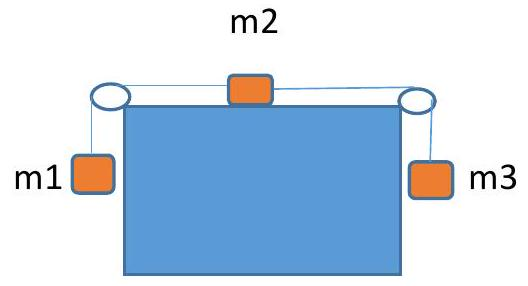
\includegraphics[max width=\textwidth, center]{2023_05_14_151379fc2bd61c0cb891g-1}
A) \(0,2 \mathrm{~g}\)
B) il sistema rimane fermo
C) \(g\)
D) \(1,04 \mathrm{~g}\)
E) \(0,5 \mathrm{~m} / \mathrm{s}^{2}\) 6) Due blocchi, \(m_{1}=10 \mathrm{~kg}\) e \(m_{2}=5 \mathrm{~kg}\) sono appesi verticalmente in serie, \(m_{1}\) al soffitto mediante il filo 1 e \(m_{2}\) a \(m_{1}\) mediante il filo 2. Supponendo i due fili inestensibili e di massa trascurabile, determinare le tensioni \(T_{1}\) (filo 1) e \(T_{2}\) (filo 2). (g = \(9.8 \mathrm{~m} / \mathrm{s}^{2}\) )
A) \(T_{1}=147 \mathrm{~N} \quad T_{2}=147 \mathrm{~N}\)
B) \(T_{1}=147 \mathrm{~N} \quad T_{2}=49 \mathrm{~N}\)
C) \(T_{1}=49 \mathrm{~N} \quad T_{2}=49 \mathrm{~N}\)
D) nessuna delle precedenti risposte

\begin{enumerate}
  \setcounter{enumi}{6}
  \item Uno scatolone avente la massa di \(50 \mathrm{~kg}\) si trova inizialmente fermo su un pavimento orizzontale scabro; il coefficiente d'attrito statico tra scatolone e pavimento è pari a 0.3. Se allo scatolone viene applicata una forza orizzontale pari a \(100 \mathrm{~N}\), costante nel tempo, allora lo scatolone
A) si muove con velocità costante
B) rimane fermo
C) si muove con accelerazione pari a \(2 \mathrm{~m} / \mathrm{s}^{2}\)
D) inizialmente si muove con velocità costante, poi accelera
E) inizialmente si muove con accelerazione costante, poi rallenta e prosegue di moto uniforme

  \item Un corpo avente la massa di \(0.15 \mathrm{~kg}\) si muove in linea retta su un piano orizzontale scabro; il coefficiente d'attrito dinamico tra corpo e piano vale 0.15. Se inizialmente il corpo possiede un'energia cinetica di \(25 \mathrm{~J}\), quanta distanza, all'incirca, percorre prima di fermarsi? \(\left(\mathrm{g}=9.8 \mathrm{~m} / \mathrm{s}^{2}\right)\)
A) \(25 \mathrm{~km}\)
B) 0.11 metri
C) \(113.4 \mathrm{~m}\)
D) 0.56 metri

\end{enumerate}

E) Non è possibile rispondere senza conoscere l'accelerazione del corpo

\begin{enumerate}
  \setcounter{enumi}{8}
  \item Su un piano orizzontale privo di attrito due forze \(\mathbf{F}_{1}=\left(-2 \mathbf{u}_{\mathbf{x}}+3 \mathbf{u}_{\mathbf{y}}\right) N\) e \(\mathbf{F}_{\mathbf{2}}=\left(-5 \mathbf{u}_{\mathbf{x}}-7 \mathbf{u}_{\mathbf{y}}\right) N\) agiscono sullo stesso corpo. Determinare il lavoro totale per uno spostamento da \(P_{1}(-7,11)\) a \(P_{2}(3,-5)\), dove le coordinate sono espresse in \(m\).
A) \(12 \mathrm{~J}\)
B) - 6 J
C) \(-10 \mathrm{~J}\)
D) \(10 \mathrm{~J}\)
E) nessuna di tali risposte è corretta

  \item Una massa \(m=102 \mathrm{~g}\), collegata ad una fune elastica \((\mathrm{k}=3.4 \mathrm{~N} / \mathrm{m})\), ruota su un piano orizzontale liscio con velocità costante \(v=5 \mathrm{~m} / \mathrm{s}\), descrivendo una circonferenza di raggio \(r=1.5 \mathrm{~m}\). Determinare l'energia meccanica totale del sistema massa-fune, sapendo che la lunghezza a riposo della fune è \(\mathrm{I}_{0}=1 \mathrm{~m}\).
A) \(12.5 \mathrm{~J}\)
B) \(1.4 \mathrm{~J}\)
C) \(1250 \mathrm{~J}\)
D) \(1.7 \mathrm{~J}\)
E) nessuna delle precedenti risposte

\end{enumerate}

\section{Punteggio:}
\begin{itemize}
  \item 3 punti per ogni risposta esatta

  \item \(\quad\) - 1 punti per ogni risposta errata

  \item 0 punti in mancanza di risposta

\end{itemize}

La prova sarà considerata superata se saranno acquisiti un minimo di 12 punti (almeno 4 risposte corrette). Per avere accesso alla prova orale, la media del punteggio di tutte le prove in itinere deve essere almeno 15.


\end{document}